\documentclass[12pt]{article}
\usepackage{amsmath}
\usepackage{graphicx}
\usepackage{enumerate}
\usepackage{natbib}
\usepackage{url}
\usepackage{enumitem}

\usepackage{amsmath,amssymb,amsthm,bm,mathtools}
\usepackage{algorithm}
\usepackage{dsfont,multirow,hyperref,setspace,enumerate}
\hypersetup{colorlinks,linkcolor={black},citecolor={black},urlcolor={black}}


\newcommand{\blind}{1}


% DON'T change margins - should be 1 inch all around.
\addtolength{\oddsidemargin}{-.5in}%
\addtolength{\evensidemargin}{-.5in}%
\addtolength{\textwidth}{1in}%
\addtolength{\textheight}{1.3in}%
\addtolength{\topmargin}{-.8in}%

\theoremstyle{definition}
\newtheorem{thm}{Theorem}[section]
\newtheorem{lem}{Lemma}
\newtheorem{prop}{Proposition}
\newtheorem{pro}{Property}
\newtheorem{cor}{Corollary}[section]

\theoremstyle{definition}
\newtheorem{assumption}{Assumption}
\newtheorem{defn}{Definition}
\newtheorem{example}{Example}
\newtheorem{rmk}{Remark}


\newtheorem{innercustomgeneric}{\customgenericname}
\providecommand{\customgenericname}{}
\newcommand{\newcustomtheorem}[2]{%
  \newenvironment{#1}[1]
  {%
   \renewcommand\customgenericname{#2}%
   \renewcommand\theinnercustomgeneric{##1}%
   \innercustomgeneric
  }
  {\endinnercustomgeneric}
}

\newcustomtheorem{customexample}{Example}

\usepackage{appendix}
\usepackage{wrapfig}
\mathtoolsset{showonlyrefs}

\usepackage{xr}
\externaldocument{jcgs-tensor}

\input macros.tex



\usepackage[english]{babel}

\newcommand*{\KeepStyleUnderBrace}[1]{%f
  \mathop{%
    \mathchoice
    {\underbrace{\displaystyle#1}}%
    {\underbrace{\textstyle#1}}%
    {\underbrace{\scriptstyle#1}}%
    {\underbrace{\scriptscriptstyle#1}}%
  }\limits
}
\usepackage{xr}


\usepackage{algpseudocode,algorithm}
\algnewcommand\algorithmicinput{\textbf{Input:}}
\algnewcommand\algorithmicoutput{\textbf{Output:}}
\algnewcommand\INPUT{\item[\algorithmicinput]}
\algnewcommand\OUTPUT{\item[\algorithmicoutput]}

\def\ci{\perp\!\!\!\perp}

\def\fixme#1#2{\textbf{\color{red}[FIXME (#1): #2]}}
\usepackage{booktabs}
\newcommand\doubleRule{\toprule\toprule}
\allowdisplaybreaks


\usepackage[compact]{titlesec}




\begin{document}



\def\spacingset#1{\renewcommand{\baselinestretch}%
{#1}\small\normalsize} \spacingset{1.5}



%%%%%%%%%%%%%%%%%%%%%%%%%%%%%%%%%%%%%%%%%%%%%%%%%%%%%%%%%%%%%%%%%%%%%%%%%%%%%%
\begin{center}
{\Large\bf Supplementary Notes to ``Supervised Tensor Decomposition
with Interactive Side Information''}
\end{center}

\appendix
\renewcommand{\thefigure}{S\arabic{figure}}
\setcounter{figure}{0}   

\section{Proofs}\label{sec:appedix}


\subsection{Proofs of Proposition~\ref{prop:alg}}\label{sec:SAlgorithm}
For notational convenience, we drop the subscript $\tY$ from the objective $\tL_\tY(\cdot)$ and simply write as $\tL(\cdot)$. Let $\tA = (\tC, \mM_1,\ldots,\mM_K) \in \mathbb{R}^{d_{\text{total}}}$ denote the collection of decision variables in the alternating optimization, where $d_{\text{total}} = \prod_k r_k + \sum_k r_kd_k$. We recall the equivalent relationship induced by orthogonal transformation.  

\begin{defn}[Equivalence class]
Two parameters $\tA'=(\tC', \mM'_1,\ldots,\mM'_k)$ and $\tA=(\tC, \mM_1,\ldots,\mM_k)$ are called equivalent, denoted $\tA\sim \tA'$, if and only if there exist a set of orthogonal matrices $\mP_k \in \mathbb{O}_{d_k,r_k}$ such that
\begin{align}\label{eq:equivalance}
	\mM'_k \mP^T_k = \mM_k ,\ \forall k \in [K], \quad \text{and}\quad \tC' \times_1 \mP_1 \times_2  \dots \times_K \mP_K = \tC.
\end{align}
\end{defn}

\begin{prop}[Global convergence]
Assume the set $\{\tA\ |\ \tL(\tA) \geq \tL(\tA^{(0)}) \}$ is compact and the stationary points of $\tL(\tA)$ are isolated module the equivalence defined in~\eqref{eq:equivalance}. Furthermore, assume that $\alpha = \infty$; i.e., we impose no entrywise bound constrains on the parameter space. Then any sequence $\tA^{(t)}$ generated by alternating algorithm converges to a stationary point of $\tL(\tA)$ module equivalence class.
\end{prop}


\begin{proof}
Pick an arbitrary iterate $\tA^{(t)}$.  Because of the compactness of set $\{\tA\colon  \tL(\tA) \geq \tL(\tA^{(0)}) \}$ and the boundedness of the decision domain, there exist a sub-sequence of $\tA^{(t)}$ that converges. Let $\tA^*$ denote one of the limiting points of $\tA^{(t)}$. Let $\tS = \{\tA^*\}$ denote the set of all the limiting points of $\tA^{(t)}$. We have $\tS \subset \{\tA\colon  \tL(\tA) \geq \tL(\tA^{(0)}) \}$ and thus $\tS$ is a compact set. By~\citet[Propositions 8.2.1 and 13.4.2]{Lange:2012:NAS:2432073}, $\tS$ is also connected. Note that all points in $\tS$ are also stationary points of $\tL(\cdot)$, because of the monotonic increase of $\tL(\tA^{(t)})$ as $t \rightarrow \infty$. 
 
 
 Consider the equivalence of Tucker tensor representation of elements in $\tS$. We define an enlarged set $\tE_S$ induced by the equivalent class of elements in $\tS$,
\begin{equation}
 \tE_S = \left\{\tA\colon \tA\sim \tA^* \text{ for some }\tA^* \in \tS\right\}.
\end{equation}
The enlarged set $\tE_S$ satisfies the two properties below:
 \begin{enumerate}
\item [1.] [Union of stationary points] The set $\tE_S$ is an union of equivalent  classes generated by the limiting points in $\tS$.
\item [2.] [Connectedness module the equivalence]  The set $\tE_S$ is connected module the equivalence relationship. That property is obtained by the connectedness of $S$.
 \end{enumerate}
Now, note that the isolation of stationary points and Property 1 imply that $\tE_S$ contains only finite number of equivalent classes. Otherwise, there is a subsequence of non-equivalent stationary points whose limit is not isolated, which contradicts the isolation assumption. Combining the finiteness with Property 2, we conclude that $\tE_S$ contains only a single equivalent class; i.e. $\tE_S = \tE_{\{\tA^*\}}$, where $\tA^*$ is a stationary point of $\tL(\tA)$. Therefore, all the convergent sub-sequences of $\tA^{(t)}$ converge to one stationary point $\tA^*$ up to equivalence. We conclude that, any iterate $\tA^{(t)}$ generated by Algorithm 1 converges to a stationary point of $\tL(\tA)$ up to equivalence.
 \end{proof}
 


\subsection{Proof of Theorem 4.1}
We restate the Theorem 4.1 from the main text. 
 \begin{thm}[Statistical convergence]\label{thm:main}
Consider a data tensor generated from supervised tensor model, where the entries are conditionally independent realizations from an exponential family. Let $(\hat \tC, \hat \mM_1,\ldots,\hat \mM_K)$ be the M-estimator and $\hat \tB=\hat \tC\times \hat \mM_1\times\cdots \times \hat \mM_K$. Define $r_\textup{total}=\prod_k r_k$ and $r_{\max}=\max_k r_k$. Under Assumptions A1 and A2 with scaled feature matrices $\check \mX_k= \sqrt{d_k}\mX_k$, or under Assumptions A1' and A2 with original feature matrices, there exist two positive constants $C_1=C_1(\alpha,K), C_2=C_2(\alpha, K)>0$ independent of dimensions $\{d_k\}$ and $\{p_k\}$, such that, with probability at least $1-\exp(-C_1\sum_k p_k)$, 
\begin{equation}\label{eq:bound}
    \FnormSize{}{\trueB- \hat \tB}^2\leq \frac{ C_{2} r_{\textup{total}}}{r_{\max}}\frac{\sum_k p_k}{\prod_k d_k}.
\end{equation}
Furthermore, if the unfolded core tensor has non-degenerate singular values at mode $k\in[K]$, i.e., $\sigma_{\min}(\textup{Unfold}_k(\tC_\textup{true})) \geq c>0$ for some constant $c$, then
\begin{equation}\label{eq:sinebound}
\textup{sin}^2 \Theta(\trueM,\ \hat \mM_k) \leq  \frac{ C_{2}r_{\textup{total}}}{ r_{\max}\sigma^2_{\min}(\textup{Unfold}_k(\tC_\textup{true}))}\frac{\sum_k p_k}{\prod_k d_k}.
\end{equation}
\end{thm}


\begin{proof}[Proof of Theorem~\ref{thm:main}]
Let $\sigma_{\text{min}}^{(k)} = \sigma_{\text{min}}(\mX_k)$ and  $\sigma_{\text{max}}^{(k)} = \sigma_{\text{max}}(\mX_k)$. First we prove \eqref{eq:bound}. 
Define $\ell(\tB)=\mathbb{E}(\tL_{\tY}(\tB))$, where the expectation is taken with respect to $\tY\sim \trueB$ under the model with true parameter $\trueB$. We prove the following two conclusions:
\begin{enumerate}
\item[C1.] There exist two positive constants $C_1$, $C_2>0$, such that, with probability at least $1-\exp(-C_1\log K\sum_k p_k)$, the stochastic deviation, $\tL_{\tY}(\tB)-\ell(\tB)$, satisfies
\[
|\tL_{\tY}(\tB)-\ell(\tB)|=|\langle \tE,\ \tB\times_1\mX_1\times_2\cdots\times_K \mX_K\rangle| \leq C_2\FnormSize{}{\tB} \left(\prod_k \sigma_{\text{max}}^{(k)}\right)\sqrt{{\prod_k r_k \over \max_k r_k} \sum_k p_k}.
\]
\item[C2.] The inequality $\ell(\hat \tB) - \ell(\trueB) \leq  -{L\over 2}\FnormSize{}{\hat \Theta-\trueT}^2$ holds, where $L>0$ is the lower bound for $\min_{|\theta|\leq \alpha}|b''(\theta)|$. 
\end{enumerate}

To prove C1, we note that the stochastic deviation based on~\eqref{eq:loglikelihood} can be written as:
\begin{align}\label{bound}
\tL_{\tY}(\tB)-\ell(\tB)&=\langle \tY-\mathbb{E}(\tY|\trueT),\ \Theta(\tB)\rangle\notag \\
&= \langle \tY- b'(\trueT),\ \Theta\rangle \notag \\
&= \langle \tE\times_1\mX^T_1\times_2\cdots\times_K\mX^T_K,\ \tB\rangle,
\end{align}
where $\tE\stackrel{\text{def}}{=}\tY-b'(\trueT)$, and the second line uses the property of exponential family that $\mathbb{E}(\tY|\tX)=b'(\trueT)$. Based on Proposition~\ref{prop}, the boundedness of $b''(\cdot)$ implies that $\tE$ is a sub-Gaussian-$(\phi U)$ tensor. Let $\check\tE\stackrel{\text{def}}{=}\tE\times_1\mX^T_1\times_2\cdots\times_K\mX^T_K$. By Proposition~\ref{prop:sub}, $\check \tE$ is a $(p_1,\ldots,p_K)$-dimensional sub-Gaussian tensor with parameter bounded by $C=\phi U\prod_k \sigma_{\text{max}}^{(k)}$. Applying Cauchy-Schwarz inequality to~\eqref{bound} yields
\begin{equation}\label{eq:bound2}
|\tL_{\tY}(\tB)-\ell(\tB)|\leq \norm{\check \tE} \nnorm{\tB},
\end{equation}
where $\norm{\cdot}$ denotes the tensor spectral norm and $\nnorm{\cdot}$ denotes the tensor nuclear norm. The nuclear norm $\nnorm{\tB}$ is  bounded by $\nnorm{\tB}\leq \sqrt{{\prod_k r_k \over \max_k r_k}}\FnormSize{}{\tB}$~\citep{wang2017operator,wang2018learning}. The spectral norm $\norm{\check \tE}$ is bounded by $\norm{\check \tE}\leq C_2\prod_k \sigma_{\text{max}}^{(k)} \sqrt{\sum_k p_k}$ with probability at least $1-\exp(-C_1\log K \sum_kp_k)$ ~\citep{tomioka2014spectral}. Combining these two bounds with~\eqref{eq:bound2}, we have, with probability at least $1-\exp(-C_1\log K \sum_kp_k)$, 
\[
|\tL_{\tY}(\tB)-\ell(\tB)|\leq C_2\FnormSize{}{\tB}\left(\prod_k \sigma_{\text{max}}^{(k)}\right)  \sqrt{ {\prod_k r_k\over \max_k r_k}\sum_k p_k},
\]
where $C_2>0$ is a constant absorbing all factors that do not depend on $\{p_k\}$ and $\{r_k\}$. 

Next we prove C2. Applying Taylor expansion to $\tL_{\tY}(\tB)$ around $\trueB$ yields
\begin{equation}\label{eq:logbefore}
\tL_{\tY}(\tB)=\tL_{\tY}(\trueB)+\Big\langle {\partial\tL_{\tY}(\tB) \over \partial
\tB}\big|_{\tB=\trueB},\tB-\trueB \Big\rangle + {1\over 2}\text{vec}(\tB-\trueB)^T \tH(\check \tB)\text{vec}(\tB-\trueB),
\end{equation}
where $\tH_{\tY}(\check \tB)$ is the (non-random) Hession of ${\partial \tL_{\tY}^2 (\tB)\over\partial^2 \tB}$ evaluated at $\check \tB = \text{vec}(\alpha \tB+(1-\alpha)\trueB)$ for some $\alpha\in[0,1]$. Note that we have used the fact that $\mathbb{E}\left({\partial\tL_{\tY}(\tB) \over \partial \tB}\big|_{\tB=\trueB}\right)=0$. This is because $\tL_{\tY}(\Theta) $ is defined as $\langle \tY,\Theta\rangle - \sum_{i_1,\ldots,i_K}b(\Theta_{i_1,\ldots,i_K})$ and
\begin{align}
{\partial \tL_\tY(\theta_{i_1,\ldots,i_K})\over \partial \theta_{i_1,\ldots,i_K}}\big|_{\Theta=\trueT}& = y_{i_1,\ldots,i_K} - {\partial b(\theta_{i_1,\ldots,i_K})\over\partial \theta_{i_1,\ldots,i_K}}\big|_{\Theta=\trueT} \\
&= y_{i_1,\ldots,i_K} - \mathbb{E}(y_{i_1,\ldots,i_K}|\theta_{i_1,\ldots,i_K\text{true}}),
\end{align}
where the last equality has used the fact that $b'(\theta) = \mathbb{E}(y|\theta)$. Taking derivative with respect to $\tB$ has the same result because of the chain rule.

We take expectation with respect to $\tY\sim \trueB$ on both sides of~\eqref{eq:log} and obtain
\begin{equation}\label{eq:log}
\ell(\tB)=\ell(\trueB)+{1\over 2}\text{vec}(\tB-\trueB)^T \tH(\check \tB)\text{vec}(\tB-\trueB).
\end{equation}
By the fact ${\partial \tL_{\tY}^2(\Theta)\over \partial^2 \Theta}=-b''(\Theta)$ and chain rule over $\Theta=\Theta(\tB)=\tB\times_1\mX_1\cdots\times_K\mX_K$, the equation~\eqref{eq:log} implies that 
\begin{equation}\label{eq:logB}
\ell(\tB)-\ell(\trueB)=-{1\over 2}\sum_{i_1,\ldots,i_K}b''(\check \theta_{i_1,\ldots,i_K}) (\theta_{i_1,\ldots,i_K}-\theta_{\text{true},i_1,\ldots,i_K})^2 \leq -{L \over 2}\FnormSize{}{\Theta-\trueT}^2,
\end{equation}
holds for all $\tB\in\tP$, provided that $\min_{|\theta|\leq \alpha}|b''(\theta)|\geq L>0$. In particular, the inequality~\eqref{eq:log} also applies to the constrained MLE $\hat \tB$. So we have
\begin{equation}\label{upper}
\ell(\hat \tB)-\ell(\trueB)\leq -{L \over 2}\FnormSize{}{\hat \Theta-\trueT}^2.
\end{equation}
Now we have proved both C1 and C2. Note that $\tL_{\tY}(\hat \tB)- \tL_{\tY}(\trueB)\geq 0$ by the definition of $\hat \tB$. This implies that
\begin{align}\label{eq:F-norm}
0&\leq \tL_{\tY}(\hat \tB)- \tL_{\tY}(\trueB) \\
&\leq \left(\tL_{\tY}(\hat \tB)-\ell(\hat \tB)\right)-\left( \tL_{\tY}(\trueB)-\ell(\trueB)\right)+\left(\ell(\hat \tB)-\ell(\trueB)\right)\\
&\leq \langle\tE,\ \Theta-\trueT    \rangle -{L\over 2}\FnormSize{}{\hat \Theta-\trueT}^2,
\end{align}
where the second line follows from~\eqref{upper}. 

The inequality~\eqref{eq:F-norm} can be rewritten as
\begin{align}\label{eq:1}
\FnormSize{}{\hat \Theta-\trueT}&\leq {2\over L}\big\langle \tE,\ {\hat \Theta -\trueT \over \FnormSize{}{\hat \Theta-\trueT}} \big\rangle\notag \\
&\leq {2\over L}\sup_{\Theta: \FnormSize{}{\Theta}=1, \Theta=\tB\times_1\mX_1\times_2\cdots\times_K \mX_K}\langle \tE,\ \Theta \rangle\notag \\
&\leq {2\over L}\sup_{\tB\in\tP: \FnormSize{}{\tB}\leq \left(\prod_k \sigma_{\min}^{(k)}\right)^{-1}} \langle \tE,\ \ \tB\times_1\mX_1\times_2\cdots\times_K\mX_K\rangle.
\end{align}
Combining~\eqref{eq:1} with C1 yields 
\begin{align}\label{eq:theta}
\FnormSize{}{\hat \Theta-\trueT} \leq {2C_2\over L} \frac{\prod_k \sigma_{\max}^{(k)}}{\prod_k \sigma_{\min}^{(k)}}\sqrt{{\prod_k r_k \over \max r_k}\sum_k p_k}.
\end{align}
Therefore,
\begin{equation}\label{eq:Bbound}
\FnormSize{}{\hat \tB-\trueB}\leq \FnormSize{}{\hat \Theta-\trueT}\left(\prod_k \sigma_{\min}^{(k)}\right)^{-1}\leq {2C_2\over L} \frac{\prod_k \sigma_{\max}^{(k)}}{\left(\prod_k \sigma_{\min}^{(k)}\right)^2}\sqrt{{\prod_k r_k \over \max r_k}\sum_k p_k}.
\end{equation}
We now consider the two cases of assumptions on the feature matrices. 
\begin{itemize}[leftmargin=0cm]
\item[] [Case 1] Under Assumption A1 with scaled feature matrices, we have the singular value
\begin{equation}\label{eq:case1}
\frac{\prod_k \sigma_{\max}^{(k)}}{\left(\prod_k \sigma_{\min}^{(k)}\right)^2} = {\prod_k c_2\sqrt{d_k}\over \left(\prod_k c_1\sqrt{d_k}\right)^2}.
\end{equation}
\item[] [Case 2] Under Assumption A1', we have asymptotic behavior of extreme singular values \citep{rudelson2010non} as 
\[
\sigma_{\text{min}}^{(k)} \sim \sqrt{d_k}-\sqrt{p_k} \text{ and  } \sigma_{\text{max}}^{(k)} \sim \sqrt{d_k}+\sqrt{p_k}.
\]
In this case, we obtain 
\begin{equation}\label{eq:case2}
\frac{\prod_k \sigma_{\max}^{(k)}}{\left(\prod_k \sigma_{\min}^{(k)}\right)^2} = {\prod_k (\sqrt{d_k}+\sqrt{p_k})\over \prod_k (\sqrt{d_k}-\sqrt{p_k})^2} =\frac{\prod_k(1+\sqrt{\gamma_k})\sqrt{d_k}}{\prod_k(1-\sqrt{\gamma_k})^2d_k}.
\end{equation}
\end{itemize}
Combining~\eqref{eq:Bbound} with either~\eqref{eq:case1} or~\eqref{eq:case2}, we obtain the same conclusion in both cases,
\[
\FnormSize{}{\hat \tB-\trueB}^2\leq \frac{ C_{2} r_{\textup{total}}}{r_{\max}}\frac{\sum_k p_k}{\prod_k d_k},
\]
where $C_2=C_2(\alpha,K,c_1, c_2)>0$ in the first case and $C_2=C_2(\alpha,K,\gamma)>0$ in the second case, both of which are constants that do not depend on the dimensions $\{d_k\}$ and $\{p_k\}$. 

Now we prove bound for sin$\Theta$ distance. 
We unfold tensors $\trueB$ and $\hat\tB$ along the mode $k$ and obtain $\text{Unfold}_k(\trueB)$ and $\text{Unfold}_k(\hat\tB)$. Notice that 
\begin{align}
    \text{Unfold}_k(\trueB) &= \mM_k \text{Unfold}_k(\trueC)\left(\mM_{k+1}\otimes\mM_{k+2}\otimes \cdots\otimes \mM_1\otimes \cdots\mM_{k-1}\right)^T,\\
    \text{Unfold}_k(\hat\tB) &= \hat\mM_k \text{Unfold}_k(\hat\tC)\left(\hat\mM_{k+1}\otimes\hat\mM_{k+2}\otimes \cdots\otimes \hat\mM_1\otimes \cdots\hat\mM_{k-1}\right)^T,
\end{align} where $\otimes$ denotes the Kronecker product of matrices.
Notice that $\mM_k$ and $\hat\mM_k$ have the same image of left singular matrices of $\text{Unfold}_k(\trueB)$ and $\text{Unfold}_k(\hat\tB)$ respectively.  Applying Proposition \ref{prop:sinebound}, we have
\begin{align}\label{eq:sintheta}
    \text{sin}^2\Theta(\mM_k,\hat\mM_k)\leq \frac{\FnormSize{}{\text{Unfold}_k(\hat\tB)-\text{Unfold}_k(\trueB)}}{\sigma_{\text{min}}(\text{Unfold}_k(\trueB))}= \frac{\FnormSize{}{\hat\tB-\trueB}}{\sigma_{\text{min}}(\text{Unfold}_k(\trueC))},
\end{align} where $\sigma_{\text{min}}(\text{Unfold}_k(\trueB)) = \sigma_{\text{min}}(\text{Unfold}_k(\trueC))$ holds based on the orthonormality of factor matrices. We finally prove the sin$\Theta$ distance by combining~\eqref{eq:sintheta} and \eqref{eq:bound}.
\end{proof}



\begin{prop}[sub-Gaussian tensors]\label{prop:sub}
Let $\tS$ be a sub-Gaussian-$(\sigma)$ tensor of dimension $(d_1,\ldots,d_K)$, and $\mX_k\in\mathbb{R}^{p_k\times d_k}$ be non-random matrices for all $k\in[K]$. Then $\tE=\tS \times_1  \mX_1\times_2\cdots\times_K  \mX_K$ is a sub-Gaussian-$(\sigma')$ tensor of dimension $(p_1,\ldots,p_K)$, where $\sigma'\leq \sigma \prod_k\sigma_{\max}(\mX_k)$. Here $\sigma_{\max}(\cdot)$ denotes the largest singular value of the matrix. 
\end{prop}

\begin{proof}
To show $\tE$ is a sub-Guassian tensor, it suffices to show that the $\tE\times_1 \bmu^T_1\times_2\cdots\times_K \bmu^T_K$ is a sub-Gaussian scalar with parameter $\sigma'$, for any unit-1 vector $\bmu_k\in\mathbb{R}^{p_k}$, $k\in[K]$. 

Note that, 
\begin{align}
\tE\times_1 \bmu^T_1\times_2\cdots\times_K \bmu^T_K&=\tS\times_1 (\bmu^T_1\mX_1) \times_2\cdots\times_K (\bmu^T_K\mX_K)\\
&= \left(\prod_k \vnormSize{}{\bmu^T_k\mX_k}\right) \KeepStyleUnderBrace{\left[\tS\times_1 { (\bmu^T_1\mX_1)\over \vnormSize{}{(\bmu^T_1\mX_1)}}\times_2\cdots\times_K { (\bmu^T_K\mX_K)\over \vnormSize{}{(\bmu^T_K\mX_K)}}\right]}_{\text{sub-Gaussian-$\sigma$ scalar}}.
\end{align}
Because $\vnormSize{}{(\bmu^T_k\mX_k)}\leq \sigma_{\max}(\mX^T_k)\vnormSize{}{\bmu_k}=\sigma_{\max}(\mX_k)$, we conclude that $\tE\times_1 \bmu^T_1\times_2\cdots\times_K \bmu^T_K$ is a sub-Gaussian tensor with parameter $\sigma \prod_k \sigma_{\max}(\mX_k)$. 
\end{proof}

\begin{prop}[sub-Gaussian residuals]\label{prop}
Define the residual tensor $\tE=\entry{\varepsilon_{i_1,\ldots,i_K}}=\tY-b'(\Theta)\in\mathbb{R}^{d_1\times \cdots \times d_K}$. Under the Assumption A2, $\varepsilon_{i_1,\ldots,i_K}$ is a sub-Gaussian random variable with sub-Gaussian parameter bounded by $\phi U$, for all $(i_1,\ldots,i_K)\in[d_1]\times\cdots\times[d_K]$.
\end{prop}
\begin{proof} The proof is similar to~\citet[Lemma 3]{fan2019generalized}. For ease of presentation, we drop the subscript $(i_1,\ldots,i_K)$ and simply write $\varepsilon$ ($=y-b'(\theta)$). For any given $t\in\mathbb{R}$, we have
\begin{align}
\mathbb{E}(\exp(t\varepsilon|\theta))&=\int c(x) \exp\left({\theta x - b(\theta)\over \phi}   \right)\exp \left(t(x-b'(\theta))\right)dx\\
&=\int c(x)\exp \left( {(\theta + \phi t)x - b (\theta+\phi t)+b(\theta+\phi t)-b(\theta)-\phi t b'(\theta) \over \phi}\right)dx\\
&=\exp\left( {b(\theta+\phi t)-b(\theta)-\phi t b'(\theta) \over \phi} \right)\\
&\leq \exp\left(\phi U t^2\over 2 \right),
\end{align}
where $c(\cdot)$ and $b(\cdot)$ are known functions in the exponential family corresponding to $y$. 
Therefore, $\varepsilon$ is sub-Gaussian-$(\phi U)$. \end{proof}

\begin{prop}[Wedin's $\sin\Theta$ Theorem]\label{prop:sinebound}
Let $\mB$ and $\hat\mB$ be two $m\times n$ real or complex with SVDs $\mB = \mU\Sigma\mV^T$ and $\hat\mB = \hat\mU\hat\mSigma\hat\mV^T.$ If $\sigma_{\text{min}}(\mB)>0$ and $\FnormSize{}{\hat\mB-\mB}\ll \sigma_{\text{min}}(\mB)$, then
\begin{align}\label{eq:sine}
    \text{sin} \Theta(\mU,\hat\mU) \leq \frac{\FnormSize{}{\hat\mB-\mB}}{\sigma_{\text{min}}(\mB)}.
\end{align}

\end{prop}
\begin{proof}
From Theorem 6.1 in \cite{wang2017tensor}, we  obtain the following bound 
\begin{align}
    \max\left\{\snormSize{}{\text{sin}\Theta(\mU,\hat\mU)},\snormSize{}{\text{sin}\Theta(\mV,\hat\mV)}\right\}\leq \frac{\max\left\{\snormSize{}{\hat\mB\mV-\mU\mSigma},\snormSize{}{\hat\mB^T\mU-\mV\mSigma}\right\}}{\sigma_{\text{min}}(\mB)}.
\end{align}
Notice that
\begin{align}
    \snormSize{}{\hat\mB\mV-\mU\mSigma} &= \snormSize{}{\hat\mB\mV-\mB\mV} = \snormSize{}{\hat\mB-\mB} \leq \FnormSize{}{\hat\mB-\mB},\\
    \snormSize{}{\hat\mB^T\mU-\mV\mSigma} &= \snormSize{}{\hat\mB^T\mU-\mB^T\mU} = \snormSize{}{\hat\mB-\mB} \leq \FnormSize{}{\hat\mB-\mB}.
\end{align}
Therefore, we prove \eqref{eq:sine}.
\end{proof}

\subsection{Proof of Corollary~\ref{thm:KL}}
\begin{proof}[Proof of Corollary~\ref{thm:KL}]
The proof is similar to~\citet{pmlr-v108-berthet20a}. We sketch the main steps here for completeness. Recall that $\ell(\tB)=\mathbb{E}(\tL_{\tY}(\tB))$. By the definition of KL divergence, we have that,
\begin{align}
\ell(\hat \tB)&=\ell(\trueB)-\sum_{(i_1,\ldots,i_K)} KL(\theta_{\text{true}, i_1,\ldots, i_K}, \hat \theta_{i_1,\ldots,i_K})\\
&=\ell(\trueB)-\text{KL}(\mathbb{P}_{\tY_{\text{true}}},\ \mathbb{P}_{\hat \tY}),
\end{align}
where $\mathbb{P}_{\tY_{\text{true}}}$ denotes the distribution of $\tY|\tX$ with true parameter $\trueB$, and $\mathbb{P}_{\hat \tY}$ denotes the distribution with estimated parameter $\hat \tB$. Therefore
\begin{align}
\text{KL}(\mathbb{P}_{\tY_{\text{true}}},\ \mathbb{P}_{\hat \tY}) &= \ell(\trueB)-\ell(\hat \tB)\\
&={1\over 2}\sum_{i_1\ldots,i_K}b''(\check \theta_{i_1,\ldots,i_K})(\theta_{i_1,\ldots,i_K}-\theta_{\text{true},i_1,\ldots,i_K})^2\\
&\leq {U\over 2} \FnormSize{}{\Theta-\trueT}^2\\
&\leq C_4{\prod_k r_k \over \max r_k}\sum_k p_k,
\end{align}
where the second line comes from~\eqref{eq:log}, and the last line is derived from~\eqref{eq:theta}. Notice that $C_4 = C(\alpha,K,U,c_1,c_2)>0$ in Assumption 1 and $C_4(\alpha,K,U,\gamma)>0$ in Assumption 1' are constants that do not depend on the dimension $\{d_k\}$ and $\{p_k\}$. 
\end{proof}

\section{Additional simulation results}
Section~\ref{sec:simulation} in the main text has provided simulation results for two settings: low-signal, high-rank setting and high-signal, low-rank setting. Here, we perform the simulations for the full combinations of rank $\mr=(3,3,3), (4,5,6)$ and signal $\alpha=3, 6$. Figures~\ref{fig:S1} and~\ref{fig:S2} confirm the outperformance of the supervised tensor method in a range of model complexities.

\begin{figure}[H]
\centering
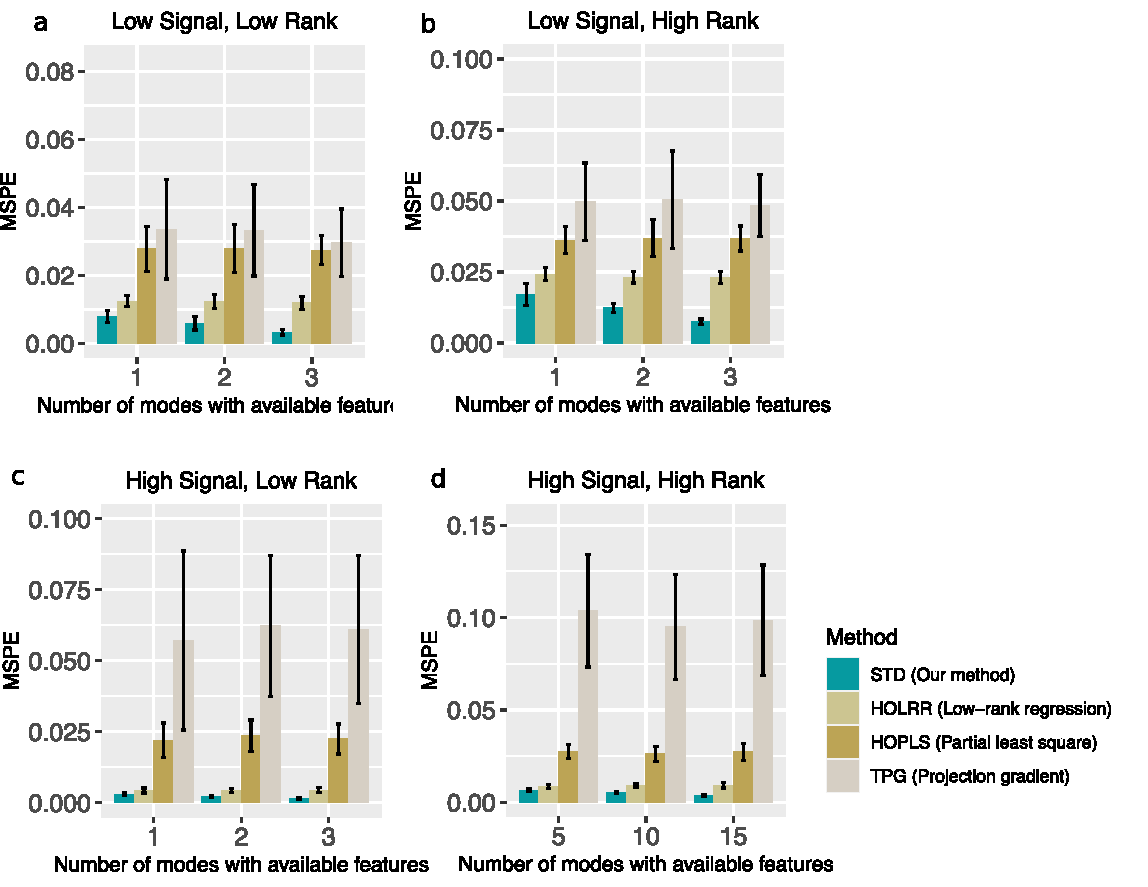
\includegraphics[width=15cm]{Supp_Figure1.pdf} 
\caption{Comparison of MSPE versus the number of modes with features. We consider full combinations of rank $\mr=(3,3,3)$ (low), $\mr=(4,5,6)$ (high), and signal $\alpha=3$ (low), $\alpha=6$ (high).}~\label{fig:S1}
\end{figure}

\begin{figure}[H]
\centering
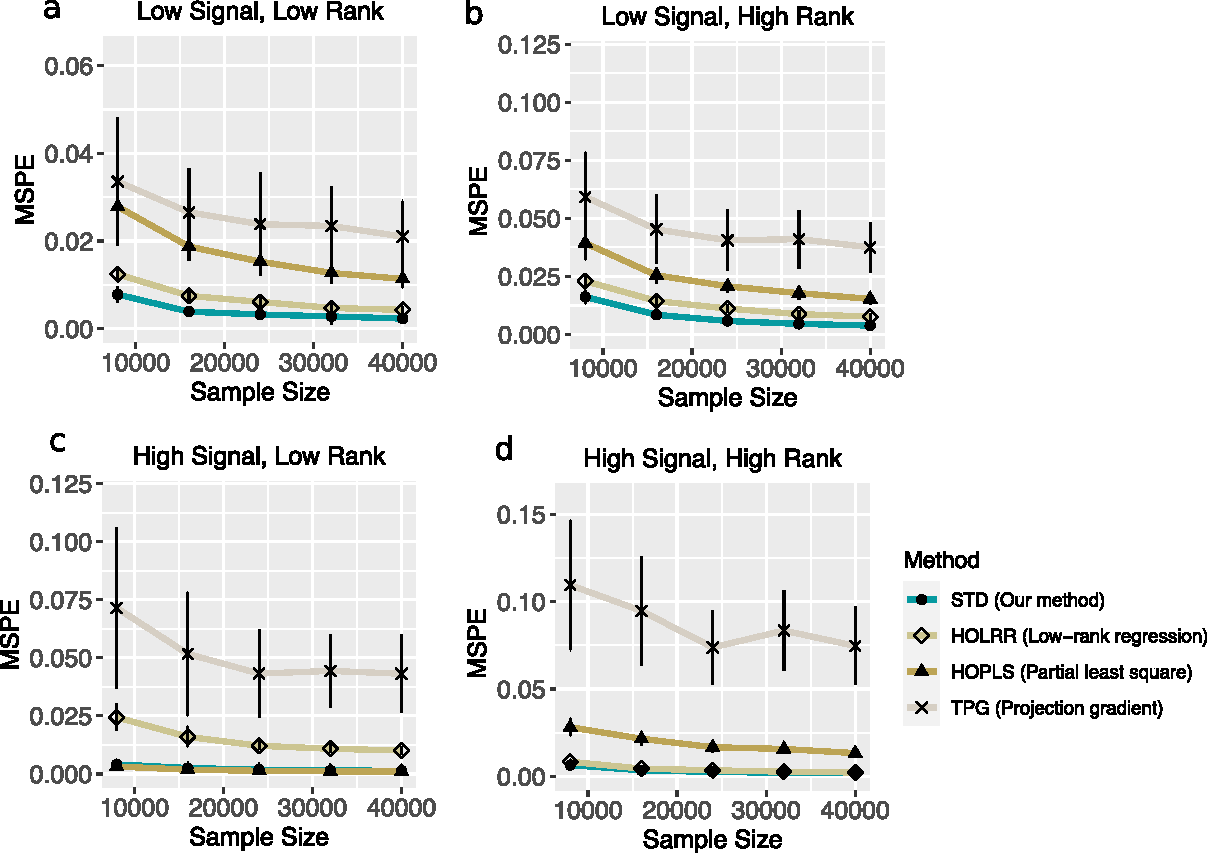
\includegraphics[width=15cm]{Supp_Figure2.pdf} 
\caption{Comparison of MSPE versus effective sample size. We consider full combinations rank $\mr=(3,3,3)$ (low), $\mr=(4,5,6)$ (high), and signal $\alpha=3$ (low), $\alpha=6$ (high). }~\label{fig:S2}
\end{figure}

\newpage
\bibliography{tensor_wang}
\bibliographystyle{apalike}


\end{document}
